%----------------------------------------------------------------------------------------
%	PACKAGES AND OTHER DOCUMENT CONFIGURATIONS
%----------------------------------------------------------------------------------------

\documentclass[
	11pt, % Set the default font size, options include: 8pt, 9pt, 10pt, 11pt, 12pt, 14pt, 17pt, 20pt
	%t, % Uncomment to vertically align all slide content to the top of the slide, rather than the default centered
	%aspectratio=169, % Uncomment to set the aspect ratio to a 16:9 ratio which matches the aspect ratio of 1080p and 4K screens and projectors
]{beamer}

% Hide navigation symbols
\setbeamertemplate{navigation symbols}{}

\usepackage{caption}
\captionsetup{labelformat=empty,labelsep=none}
\graphicspath{{images/}{./}} % Specifies where to look for included images (trailing slash required)
\usepackage{minted}
% \usepackage{setspace}
\linespread{1}
\usepackage{amsmath}
\usepackage{multirow}
\usepackage{color, colortbl}
\usepackage{xcolor}
\usepackage{booktabs} % Allows the use of \toprule, \midrule and \bottomrule for better rules in tables
\usepackage{graphicx}
\usepackage{minibox}
\renewcommand{\arraystretch}{1.2} % Default value: 1
\definecolor{darkGreen}{RGB}{9,150,3} 
\usepackage{tikz}

\newcommand{\tikzunderarrow}[2][black]{\tikz[baseline={(N.base)}]{
  \node[inner sep=0, outer sep=0](N) {#2};
  \draw[overlay, -latex, line width=.04em, #1]
    ([yshift=-.14em]N.south west) -- ([yshift=-.14em]N.south east);}}
\usepackage{ragged2e}
\tolerance=1
\emergencystretch=\maxdimen
\hyphenpenalty=10000
\hbadness=10000

%----------------------------------------------------------------------------------------
%	SELECT LAYOUT THEME
%----------------------------------------------------------------------------------------

% Beamer comes with a number of default layout themes which change the colors and layouts of slides. Below is a list of all themes available, uncomment each in turn to see what they look like.

%\usetheme{default}
%\usetheme{AnnArbor}
%\usetheme{Antibes}
%\usetheme{Bergen}
%\usetheme{Berkeley}
% \usetheme{Berlin}
%\usetheme{Boadilla}
% \usetheme{CambridgeUS}
% \usetheme{Copenhagen}
% \usetheme{Darmstadt}
% \usetheme{Dresden}
% \usetheme{Frankfurt}
% \usetheme{Goettingen}
% \usetheme{Hannover}
% \usetheme{Ilmenau}
% \usetheme{JuanLesPins}
% \usetheme{Luebeck}
\usetheme{Madrid}
%\usetheme{Malmoe}
%\usetheme{Marburg}
%\usetheme{Montpellier}
%\usetheme{PaloAlto}
%\usetheme{Pittsburgh}
%\usetheme{Rochester}
%\usetheme{Singapore}
%\usetheme{Szeged}
%\usetheme{Warsaw}

%----------------------------------------------------------------------------------------
%	SELECT COLOR THEME
%----------------------------------------------------------------------------------------

% Beamer comes with a number of color themes that can be applied to any layout theme to change its colors. Uncomment each of these in turn to see how they change the colors of your selected layout theme.

% \usecolortheme{albatross}
% \usecolortheme{beaver}
% \usecolortheme{beetle}
% \usecolortheme{crane}
% \usecolortheme{dolphin}
% \usecolortheme{dove}
% \usecolortheme{fly}
% \usecolortheme{lily}
% \usecolortheme{monarca}
% \usecolortheme{seagull}
% \usecolortheme{seahorse}
\usecolortheme{spruce}
% \usecolortheme{whale}
% \usecolortheme{wolverine}

%----------------------------------------------------------------------------------------
%	SELECT FONT THEME & FONTS
%----------------------------------------------------------------------------------------

% Beamer comes with several font themes to easily change the fonts used in various parts of the presentation. Review the comments beside each one to decide if you would like to use it. Note that additional options can be specified for several of these font themes, consult the beamer documentation for more information.

\usefonttheme{default} % Typeset using the default sans serif font
%\usefonttheme{serif} % Typeset using the default serif font (make sure a sans font isn't being set as the default font if you use this option!)
\usefonttheme{structurebold} % Typeset important structure text (titles, headlines, footlines, sidebar, etc) in bold
%\usefonttheme{structureitalicserif} % Typeset important structure text (titles, headlines, footlines, sidebar, etc) in italic serif
%\usefonttheme{structuresmallcapsserif} % Typeset important structure text (titles, headlines, footlines, sidebar, etc) in small caps serif

%------------------------------------------------

%\usepackage{mathptmx} % Use the Times font for serif text
\usepackage{palatino} % Use the Palatino font for serif text

%\usepackage{helvet} % Use the Helvetica font for sans serif text
\usepackage[default]{opensans} % Use the Open Sans font for sans serif text
%\usepackage[default]{FiraSans} % Use the Fira Sans font for sans serif text
%\usepackage[default]{lato} % Use the Lato font for sans serif text

%----------------------------------------------------------------------------------------
%	SELECT INNER THEME
%----------------------------------------------------------------------------------------

% Inner themes change the styling of internal slide elements, for example: bullet points, blocks, bibliography entries, title pages, theorems, etc. Uncomment each theme in turn to see what changes it makes to your presentation.

%\useinnertheme{default}
\useinnertheme{circles}
% \useinnertheme{rectangles}
% \useinnertheme{rounded}
%\useinnertheme{inmargin}

%----------------------------------------------------------------------------------------
%	SELECT OUTER THEME
%----------------------------------------------------------------------------------------

% Outer themes change the overall layout of slides, such as: header and footer lines, sidebars and slide titles. Uncomment each theme in turn to see what changes it makes to your presentation.

% \useoutertheme{default}
% \useoutertheme{infolines}
\useoutertheme{miniframes}
% \useoutertheme{smoothbars}
% \useoutertheme{sidebar}
%\useoutertheme{split}
% \useoutertheme{shadow}
% \useoutertheme{tree}
%\useoutertheme{smoothtree}

%\setbeamertemplate{footline} % Uncomment this line to remove the footer line in all slides
%\setbeamertemplate{footline}[page number] % Uncomment this line to replace the footer line in all slides with a simple slide count

%\setbeamertemplate{navigation symbols}{} % Uncomment this line to remove the navigation symbols from the bottom of all slides

%----------------------------------------------------------------------------------------
%	PRESENTATION INFORMATION
%----------------------------------------------------------------------------------------

\title[LAB 08: MIPS Exceptions and I/O]{LAB 08: MIPS Exceptions and I/O} % The short title in the optional parameter appears at the bottom of every slide, the full title in the main parameter is only on the title page

% \subtitle{Optional Subtitle} % Presentation subtitle, remove this command if a subtitle isn't required

\author[S. AlSaleh]{Saleh AlSaleh \\ \smallskip \textit{salehs@kfupm.edu.sa}} % Presenter name(s), the optional parameter can contain a shortened version to appear on the bottom of every slide, while the main parameter will appear on the title slide

\institute[KFUPM]{King Fahd University of Petroleum and Minerals \\ College of Computing and Mathematics \\ Computer Engineering Department} % Your institution, the optional parameter can be used for the institution shorthand and will appear on the bottom of every slide after author names, while the required parameter is used on the title slide and can include your email address or additional information on separate lines

\date[March 05, 2023]{COE301: Computer Architecture \\ Term 222} % Presentation date or conference/meeting name, the optional parameter can contain a shortened version to appear on the bottom of every slide, while the required parameter value is output to the title slide

%----------------------------------------------------------------------------------------

\begin{document}

%----------------------------------------------------------------------------------------
%	TITLE SLIDE
%----------------------------------------------------------------------------------------

\begin{frame}
	% Output the title slide, automatically created using the text entered in the PRESENTATION INFORMATION block above
	\titlepage
\end{frame}

%----------------------------------------------------------------------------------------
%	TABLE OF CONTENTS SLIDE
%----------------------------------------------------------------------------------------

% The table of contents outputs the sections and subsections that appear in your presentation, specified with the standard \section and \subsection commands. You may either display all sections and subsections on one slide with \tableofcontents, or display each section at a time on subsequent slides with \tableofcontents[pausesections]. The latter is useful if you want to step through each section and mention what you will discuss.

\begin{frame}
	\frametitle{Agenda} % Slide title, remove this command for no title
	
	\tableofcontents % Output the table of contents (all sections on one slide)
	%\tableofcontents[pausesections] % Output the table of contents (break sections up across separate slides)
\end{frame}

%----------------------------------------------------------------------------------------
%	PRESENTATION BODY SLIDES
%----------------------------------------------------------------------------------------

\section{Exceptions} % Sections are added in order to organize your presentation into discrete blocks, all sections and subsections are automatically output to the table of contents as an overview of the talk but NOT output in the presentation as separate slides
\begin{frame}
	\frametitle{Exceptions}
	
	\begin{itemize}
		\item Exception is any unexpected change of control flow, regardless of its source. \pause 
		\item MIPS CPU operates either in the user mode or kernel mode. \pause
		\item User programs (applications) run in user mode. \pause
		\item The CPU enters the kernel mode when an exception happens/occurs. \pause
		\item In MIPS, all the instructions inside text segment are in the try block.
	\end{itemize}

\end{frame}

%------------------------------------------------


\begin{frame}
	\frametitle{Coprocessor 0}
	\begin{itemize}
		\item Coprocessor 0 has several important registers such as:
		\begin{itemize}
			\item \textbf{Vaddr (\color{red}\$8\color{black})}: Contains the invalid memory address caused by load, store, or fetch. \pause
			\item \textbf{Status (\color{red}\$12\color{black})}: Contains the interrupt mask and enable bits. \pause
			\item \textbf{Cause (\color{red}\$13\color{black})}: Contains the type of exception and any pending bits (see below). \pause
			\item \textbf{EPC (\color{red}\$14\color{black})}: Contains the address of the instruction when the exception occurred. \pause
		\end{itemize}
	\end{itemize}
	\begin{figure}
		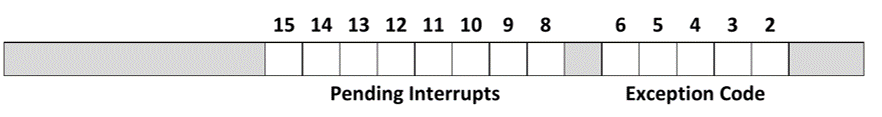
\includegraphics[width=\linewidth]{cause_register.png}
		\caption{The \textbf{Cause} Register \textbf{\$13}}
	\end{figure}
\end{frame}


\begin{frame}
	\frametitle{Exception Codes}
	Common Exception Codes for MIPS
	\begin{table}
		\centering
		\resizebox{\linewidth}{!}{%
			\begin{tabular}{|l|l|l|}
				\toprule
				\textbf{Code} 	& \textbf{Name} & \textbf{Description} 															\\
				\midrule
				0   			& INT           & Hardware Interrupt															\\ \hline
				4   			& ADDRL         & Address error exception caused by load or instruction fetch					\\ \hline
				5   			& ADDRS     	& Address error exception caused by store										\\ \hline
				6   			& IBUS     		& Bus error on instruction fetch												\\ \hline
				7   			& DBUS    		& Bus error on data load or store												\\ \hline
				8   			& SYSCALL    	& System call exception caused by the \textbf{syscall} instruction				\\ \hline
				9   			& BKPT    		& Breakpoint exception caused by the \textbf{break} instruction					\\ \hline
				10  			& RI    		& Reserved instruction exception												\\ \hline
				12  			& OVF           & Arithmetic overflow exception													\\ \hline
				13  			& TRAP          & Exception caused by a trap instruction										\\ \hline
				15  			& FPE           & Floating-Point exception cause by a floating-point instruction				\\ 
				\bottomrule
			\end{tabular}%
		}
	\end{table}
\end{frame}


\begin{frame}
	\frametitle{Exception Handler}
	\begin{columns}[c]
		\begin{column}{0.5\textwidth}
			\begin{itemize}
				\item A special piece of code in the kernel text (at address \textbf{0x80000180}) that handles exceptions. \pause
				\item There is a default exception handler in MARS. However, it can be overwritten. \pause
			\end{itemize}
		\end{column}
	
		\begin{column}{0.5\textwidth}
			\begin{figure}
				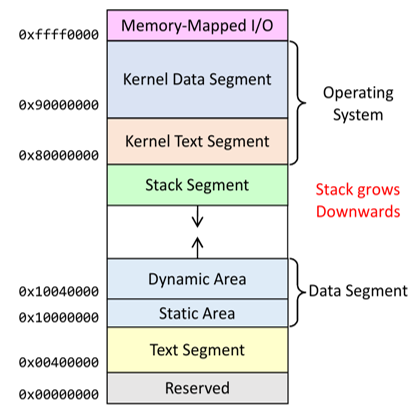
\includegraphics[width=\linewidth]{mips_memory_exception.png}
				\caption{MIPS Memory Organization}
			\end{figure}
		\end{column}
	\end{columns}
\end{frame}

%------------------------------------------------

\section{Memory Mapped I/O}
\begin{frame}
	\frametitle{Memory Mapped I/O}
	\begin{columns}[c]
		\begin{column}{0.5\textwidth}
			\begin{itemize}
				\item Input/Output devices reside outside the processor chip. \pause
				\item There are two general ways for the processor to communicate with the I/O devices:
				\begin{itemize}
					\item Using specialized instruction to communicate with each device. \pause
					\item Map I/O device registers to memory space. Then, use load and store instructions to read and write to the devices respectfully. \pause
				\end{itemize}
			\end{itemize}
		\end{column}
		\begin{column}{0.5\textwidth}
			\begin{figure}
				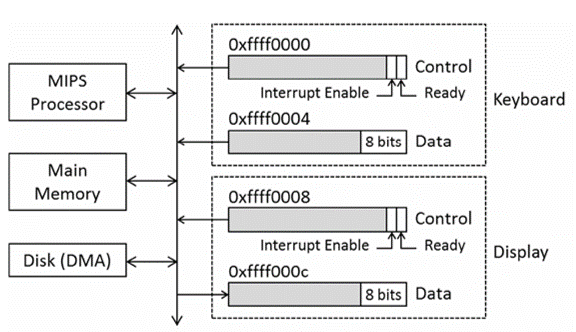
\includegraphics[width=\linewidth]{mmio.png}
				\caption{MIPS Memory Mapped I/O}
			\end{figure}
		\end{column}
	\end{columns}
\end{frame}

%------------------------------------------------

\section{Live Examples}

\begin{frame}
	\frametitle{Live Examples}
	
\end{frame}

%------------------------------------------------

\section{Tasks}

\begin{frame}
	\frametitle{Task \#1}
	\begin{columns}[c]
		\begin{column}{0.4\textwidth}
			\justifying
			Write a MIPS assembly program that reads two integers from the user \textbf{x} and \textbf{y}. If y is zero, raise an exception and the user should be prompted to enter a different value of y. If y is not zero, perform the operation x/y. 

			(Hint: use trap instruction after reading y)
		\end{column}
		\begin{column}{0.6\textwidth}
		\centering
			\centering
			Sample Run 

			\minibox[frame,pad=4pt]{
				\color{black}Enter Dividend (x): \color{blue}10 \\
				\color{black}Enter Divisor (y): \color{blue}0 \\
				Divide By Zero Exception.\\
				Please enter a different value for y.\\
				\color{black}Enter Divisor (y): \color{blue}2 \\
				\color{black}The result of x/y is \color{darkGreen}5 \\
			}
			
		\end{column}
	\end{columns}
\end{frame}
\begin{frame}
	\frametitle{Task \#2}
	\begin{columns}[c]
		\begin{column}{0.7\textwidth}
			\justifying
			Write a MIPS assembly program that reads a string str (one character at a time) from the user using Memory Mapped I/O (\color{red}DO NOT USE syscall\color{black}). Loop over each character and flip its case (i.e. the uppercase should be small case and vice versa). Finally, print the modified String (one character at a time) again using Memory Mapped I/O (\color{red}DO NOT USE syscall\color{black}).
		\end{column}
		\begin{column}{0.3\textwidth}
		\centering
			\centering
			Sample Run 

			\minibox[frame,pad=4pt]{
				\color{blue}Hello, World!				\\
				\color{darkGreen}hELLO, wORLD!			\\
			}
			
		\end{column}
	\end{columns}
\end{frame}

%----------------------------------------------------------------------------------------

\end{document} 